\documentclass[12pt]{article}
\usepackage[utf8]{inputenc}
\usepackage{xcolor}
\usepackage{graphicx}
\usepackage{listings}
\usepackage{epstopdf}
\usepackage{etoc}
\usepackage{pdfpages}
\usepackage[capposition=top]{floatrow}
\usepackage{pdflscape} % landsacpe package
% set font to times
%\usepackage{mathptmx} % times!!! 
%\usepackage[T1]{fontenc}
\usepackage{amsmath}
\usepackage{soul}
\usepackage[left=2.5cm, right=2.5cm, top=2.5cm, bottom =2.5cm]{geometry}
\usepackage{natbib}
%\usepackage[natbibapa]{apacite}
%\usepackage{apacite}
%\bibliographystyle{apacite}
\bibliographystyle{apa}
%\renewcommand{\footnotesize}{\fontsize{10pt}{11pt}\selectfont}
\usepackage[onehalfspacing]{setspace}
\usepackage{listings}
\renewcommand{\figurename}{\textbf{Figure}}
\renewcommand{\hat}{\widehat}
\usepackage[bf]{caption}
\usepackage{tikz}
%\begin{comment}
%\usepackage[headsepline,footsepline]{scrlayer-scrpage} % has to come before package!!! otherwise option clash
%\usepackage{scrlayer-scrpage}
%\pagestyle{scrheadings} % kopfzeile/ fußzeile
%\clearpairofpagestyles
%\ohead{}
%\ihead{\textit{Redistribution, Demand and  Sustainable Production}}
%\cfoot{\thepage}
%\pagestyle{plain} % comment this one to have header
%\end{comment}
\usepackage{comment}
 \usepackage{siunitx}
  \usepackage{textcomp}
\definecolor{sonja}{cmyk}{0.9,0,0.3,0}
%\definecolor{purple}{model}{color-spec}
\usepackage{amssymb}
\newcommand{\ar}{$\Rightarrow$ \ }
\newcommand{\frp}[2]{\frac{\partial{#1}}{\partial{#2}}}
\newcommand{\tr}[1]{\textcolor{red}{#1}}
\newcommand{\vlt}[1]{\textcolor{violet}{#1}}
\newcommand{\bl}[1]{\textcolor{blue}{#1}}
\newcommand{\sn}[1]{\textcolor{sonja}{#1}}
%%% TIKZS
\usepackage{tikz}
\usetikzlibrary{mindmap,trees}
\usetikzlibrary{backgrounds}
\tikzstyle{every edge}=  [fill=orange]  
\usetikzlibrary{tikzmark}
\usetikzlibrary{decorations.markings}
\usepackage{tikz-cd}
\usetikzlibrary{arrows,calc,fit}
\tikzset{mainbox/.style={draw=sonja, text=black, fill=white, ellipse, rounded corners, thick, node distance=5em, text width=8em, text centered, minimum height=3.5em}}
\tikzset{mainboxbig/.style={draw=sonja, text=black, fill=white, ellipse, rounded corners, thick, node distance=5em, text width=13em, text centered, minimum height=3.5em}}
\tikzset{dummybox/.style={draw=none, text=black , rectangle, rounded corners, thick, node distance=4em, text width=20em, text centered, minimum height=3.5em}}
\tikzset{box/.style={draw , rectangle, rounded corners, thick, node distance=7em, text width=8em, text centered, minimum height=3.5em}}
\tikzset{container/.style={draw, rectangle, dashed, inner sep=2em}}
\tikzset{line/.style={draw, very thick, -latex'}}
\tikzset{    pil/.style={
		->,
		thick,
		shorten <=2pt,
		shorten >=2pt,}}
	
% other stuff
\newcommand{\innermid}{\nonscript\;\delimsize\vert\nonscript\;}
\newcommand{\activatebar}{%
	\begingroup\lccode`\~=`\|
	\lowercase{\endgroup\let~}\innermid 
	\mathcode`|=\string"8000
}
%\usepackage{biblatex}
%\addbibresource{bib_mt.bib}
\usepackage{ulem}
\title{Growth, the Environment, and Inequality\\ \small{ reduction policies in an endogenous growth model with inequality}}
\date{Sonja Dobkowitz\\ Bonn Graduate School of Economics\\ %University of Bonn\\
\vspace{1mm}
%Preliminary and incomplete\\
First version: December 15, 2021\\
This version: \today }
\usepackage{graphicx,caption}
\usepackage{hyperref}
\usepackage{minitoc}
\setcounter{secttocdepth}{5}
\usetikzlibrary{shapes.geometric}

% for tabular

%\usepackage{array}
\usepackage{makecell}
\usepackage{multirow}
\usepackage{bigdelim}

\renewenvironment{abstract}
{\small
	\list{}{
		\setlength{\leftmargin}{0.025\textwidth}%
		\setlength{\rightmargin}{\leftmargin}%
	}%
	\item\relax}
{\endlist}
\begin{document}
%	\includepdf[pages=-]{../titlepage.pdf}
	\maketitle
	
\section{Timeline}
\begin{itemize}
	\item check difference to \cite{Acemoglu2016TransitionTechnology} 17/12 \checkmark
\item by Saturday 18/12: have solved model as in AA solved analytically
\item read Aghion paper on social responsibility
\item by Monday 19/12: understand code
\item xxx: model extension with clean sector causing externality 
\item[\ar] what is the effect on the optimal policy as compared to AA
\item add working time reduction as policy
\end{itemize}

\section{Fields connected by the project}
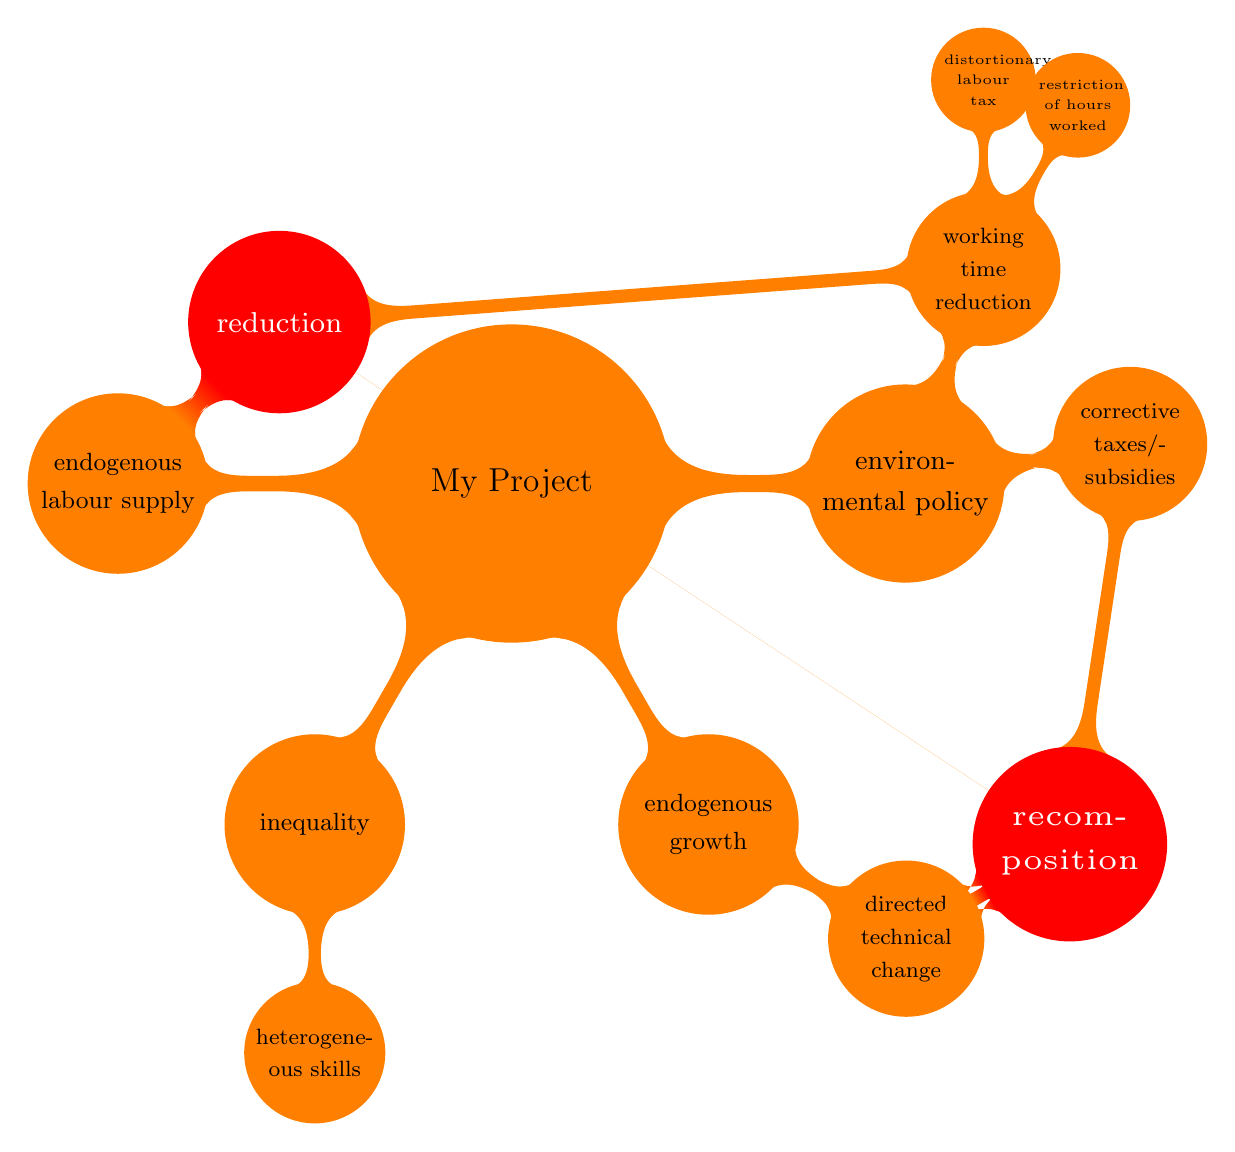
\begin{tikzpicture}[]
\path[mindmap,concept color=orange,text=black]
node[concept] {My Project}
[clockwise from=0]
child[] {
	node[concept, scale=1.1] {environ- mental policy}
	[clockwise from=70]
	child { node[concept] (wtr)  {working time reduction} [clockwise from=90]
		child {node[concept] {distortionary labour tax}}
		child {node[concept, level distance=2cm] {restriction of hours worked}}
	}
	child { node[concept] (corr) {corrective taxes/subsidies}
	}
}  
child[concept color=orange] {
	node[concept] (endg) {endogenous growth}
	[clockwise from=-30]
	child { node[concept] (dtc) {directed technical change} 
		[clockwise from=30, level distance=10cm]
child [ concept color=red, text=white] { node[concept,  scale=2.1] (recomposition) {recom- position} }	
}
}
child[concept color=orange] { node[concept] {inequality} 
	[clockwise from=-90]
	child { node[concept] (hetskill) {heterogene-  ous skills}} 
}
child[concept color=orange] { node[concept] (endlab) {endogenous labour supply} [clockwise from=45]
	child [ concept color=red, text=white] { node[concept, scale=1.3] (reduc) {reduction}} 
};

\begin{pgfonlayer}{background}
\draw [circle connection bar ]
(recomposition) edge (corr) [color=orange]
(reduc) edge (wtr) [color=orange];
\end{pgfonlayer}


\draw[->,  black] (reduc) edge (recomposition);

\end{tikzpicture}

\section{Motivation}
\subsection{From Directed Technical Change direction}
%\tr{a gradual approach and not categorised}
\paragraph{introduce two policies: complements and interlinked}
Planetary boundaries are violated or threatened to be by human activity \citep{Rockstrom2009AHumanity}. The need to reduce environmental externalities of production becomes more and more vital.  % why this?/ Resource consumption= to emissions??? 
Two measures to lower environmental externalities feature prominently in the discussion: a recomposition and a reduction approach. Macroeconomic research by and large has focused on the former: instead of producing a high share of polluting goods the optimal policy directs resources to the clean sector. Models of directed technical change, in particular, are designed to study recomposition through policies and market forces.
Proponents of a reduction approach question the possibility that a recomposition of production alone suffices to meet planetary boundaries. The two approaches are most likely (i) complements to keep the environment in an inhabitable state and (ii) interlinked through general equilibrium effects. However,
a joint macroeconomic analysis of both policies is hitherto missing. 

\tr{The next to paragraphs are 2 options on how to continue. Either with distortionary taxes (Version 1) or with working time reductios (Version 2); }
\paragraph{Version 1: what I do: With distortionary labour tax or general consumption tax}
To fill this gap, I present a model of directed technical change in which no perfectly clean technology can be innovated. Therefore, a reduction policy might be inevitable. Having distortionary labour taxes at its disposal, the government has the means to reduce economic output overall. A reduction in output directly lowers the externality. However, I argue, that reduction policies and the direction of technical growth are interrelated through inequality. 


 This indirect channel might undermine the direct advantageous effect of a reduction policy on the externality. It is, therefore, questionable whether they are part of the optimal policy.

\paragraph{Version 2: what I do: with restriction of maximum working hours}
To fill this gap, I present a model of directed technical change in which no perfectly clean technology can be innovated. Therefore, a reduction policy might be inevitable. As put forward by the literature advocating reduction policies, the government in the model can restrict the maximum hours worked per employee \textit{(consult \cite{Schor2005SustainableReduction})}.\footnote{\ One rationale behind working hour restrictions as a tool to reduce production is that this policy faces more acceptance in society than higher income or consumption taxes \citep[e.g.][]{Schor2005SustainableReduction, Alvarez-Cuadrado2007EnvyHours}.}
This tool allows the government to reduce output overall which lowers the externality directly.
However, a decline in demand and labour supply may discourage incentives to innovate in the cleaner sector. This indirect channel might undermine the direct advantageous effect on the externality. It is, therefore, questionable whether they are part of the optimal policy.

\paragraph{Adding inequality}
We live in a time characterised by high degrees of inequality. I argue that this aspect of today's economies crucially determines the mechanisms of environmental policies in market economies. Empirical research has provided evidence for a skill bias in cleaner sectors of production \citep{Consoli2016DoCapital}. Assume the government cannot differentiate households by skill and raises the labour tax for all households. Especially high-skilled households might reduce their labour supply if they are richer \textit{(need to find evidence for this: income share of high skilled)} due to a lower shadow value of income \textit{(have to differentiate substitution and income channel here)}. This again lowers the market size of the cleaner sector thereby dampening clean innovation incentives. On the other hand, the price of the cleaner good might rise more than that of the dirty good. Through the price effect clean innovation could accelerate again. Hence, accounting for skill heterogeneity across sectors adds to the ambiguous effect of reduction policies on recomposition policies.


\paragraph{ Research Question (What)}

The interrelationship of reduction, recomposition, and inequality motivates to ask: What is the optimal environmental policy? 


\subsection{Alternative motivation coming from the optimal taxation literature}
The public finance literature has focused the discussion of optimal labour income taxation and the degree of progressivity on the equity-efficiency trade-off.  The benefits of labour taxes arise from redistribution. With concave utility specifications full redistribution is efficient. However, the optimal tax system does not feature full redistribution when labour supply is endogenous. Instead, the degree of redistribution is traded-off against aggregate output as individuals reduce their labour supply in response to the labour income tax. 

\paragraph{An environmental perspective}
 Adding environmental externalities to the classical public finance framework may change the light with which efficiency costs are perceived. Instead of merely reducing welfare, direct benefits through output reduction arise by lowering the externality. 

In general, the presence of corrective tax instruments, which direct production to a non-polluting alternative, however, distortionary labour taxes are not employed as environmental policy instruments under standard preferences.\footnote{ Compare my paper on Sustainable production and demand where there is no limit/ no disaster.} This finding depends on how the externality is modeled. Indeed, some (non-economist) scholars argue for the necessity to reduce current consumption levels in developed economies in the light of threats to planetary boundaries. This can be understood by the pressing time frame to correct for climate externalities in particular and serious threats to other planetary boundaries \citep{Rockstrom2009AHumanity}\footnote{\ In their article, \cite{Rockstrom2009AHumanity} argue that several planetary boundaries have already been surpassed. Uncertainties about their interaction are another argument in favour of more cautious environmental policies. } such as biodiversity and nitrogen xxx.
Taken this broader view on environmental pollution through economic activity, it becomes more questionable, if a perfectly clean technology exists or can ever be innovated.  

In sum, the need to reduce environmental externalities rather quickly and the potential non-existence of perfectly green technologies could render classical fiscal tax instruments environmental policy tools through the efficiency channel. 

\textit{So far: efficiency-equity channel; plus on efficiency side}
\paragraph{Trade-offs: environmental externality}
While having an advantageous direct effect on the externality, counteracting indirect effects arise in a general equilibrium framework. Proponents of a reduction policy especially focus on consumption by the rich which consume a higher amount of natural resources.\footnote{\ Note Sonja: Abstracting from inequality, would it still be best to reduce consumption by the rich when the poor have a higher marginal propensity to consume dirty? \textit{Could be an important aspect in the model}.}
This concern could add to the benefits of tax progressivity.
However, targeting these households in particular for environmental reasons, in contrast, will lower high skill labour supply and investment into it. Yet, these skills are especially used in green sectors of the economy \citep{Consoli2016DoCapital}. As a result, dirty production becomes relatively cheaper and the dirty share of production rises. 

The literature on optimal environmental policy knows the 
Furthermore, the direction of technological change might be drawn towards the more polluting good in response to a higher progressivity. The reduction in the cleaner sector's labour input good diminishes the relative market size of this sector. The market effect shifts innovation towards the bigger dirty sector. On the other hand, the higher price of the clean sector makes innovation in the clean sector more profitable, the price effect. 
One contribution of the paper is to discuss optimal fiscal policy in an endogenous growth setting. 

Given these counteracting forces, this paper seeks to answer whether a reduction policy is indeed optimal for environmental reasons. 
\\

\noindent\rule[1ex]{\textwidth}{1pt}
\paragraph{The below is an addendum in case I want to add capital taxation somewhere...} \tr{below relatively close to \cite{Conesa2009TaxingAll}} 
Another prominent debate in the public finance literature centres on the optimal size of the capital tax. The optimality of zero capital taxation has been argued for in the seminal work by Judd (1985) and affirmed by others.  However, as discussed by \cite{Conesa2009TaxingAll}, the optimality of a zero capital tax hinges upon the endogeneity of labour supply. The capital tax rises when allowing for life-cycle aspects. In this setting, it is optimal to tax capital heavily and to accept a reduction in consumption at a modest reduction of hours worked for the benefit of better insurance and redistribution. Taking environmental externalities into account, the optimal capital tax may even be higher due to its advantageous effect on the externality.

\cite{Domeij2004OnTaxes} discuss a reduction of capital taxes in a model with idiosyncratic productivity shocks which imply  wealth inequality. Their focus rests on the distributional effect which arise in the transition from the benchmark to a lower capital tax. They find huge negative distributional effects over the transition since a linear labour tax is less progressive.  (\textit{check this}) The distributional effects outweigh the benefits of a higher capital stock and output. 
\\

\noindent\rule[1ex]{\textwidth}{1pt}

\paragraph{Empirical motivation}
The key channel in the paper which induces adverse consequences of a reduction policy on the externality hinges on the skill-bias in the cleaner sector and that consumption-rich households are high skill households. I document a positive correlation between skills and sectors and between income and skills building on xxx data.

\paragraph{Exercise}
First, I study the effects of labour-tax progressivity  on the environmental externality in a tractable general equilibrium model with directed technical change. The model builds on \cite{Heathcote2017OptimalFramework} and \cite{Acemoglu2012TheChange}. 
In contrast to \cite{Heathcote2017OptimalFramework}, I abstract from idiosyncratic risk to focus on the medium to long run. 
The planner still faces the trade-off between equity and skill accumulation. 
In this part of the paper, I focus on conditions on the processes shaping the relation of production and the environment so that fiscal policies are employed for environmental reasons although corrective taxes are available.  

Second, in a quantitative analysis, I examine the optimal policy and transitions to the new steady state from a realistically calibrated current state of the economy. Two possible setups seem interesting. (1) The government maximises a \textit{(possibly pareto-weighted, utilitarian)} social welfare function. (2, \textit{if I only focus on carbon}) The government takes the climate target of the Paris agreement as constraint while maximising a social welfare function.  
To scrutinise the contribution of directed technological change and skill heterogeneity, I rerun the analysis in versions of the model where either or both channels are shut down. In order to understand why the optimal policy in the benchmark model differs from the simplified versions, I introduce the optimal policy in e.g. the version without skill heterogeneity into the full model. The difference between the two model is driven by inequality. 
\\

\noindent\rule[1ex]{\textwidth}{1pt}
\noindent \textbf{Alternative sequence of quantitative exercises, seems a better fit when analytical stuff doesn't work out}
\begin{enumerate}
	\item[-] two sector model with no perfectly clean technology
	\item[-] government chooses capital tax, progressivity of labour tax, consumption tax, corrective tax
	\item representative agent no endogenous innovation: what is the optimal policy?
	\item add separately 
	\begin{enumerate}
		\item heterogeneity in skills (first, as it is closer to optimal policy literatue!)
		\item endogenous innovation
	\end{enumerate}
and (1) impose the optimal policy under the rep agent, (2) what is the optimal policy in each?
\item add all together
\item[-] focus analysis on effects on externality (or/and standard welfare measure for comparison)
\item \textbf{sensitivity: look at different utility specifications (a) habits/social preferences, (b) non-homothetic preferences, income-dependent marginal propensities to consume polluting goods (use first paper's preferences), (c) social profit of leisure}
\end{enumerate}

\subsection{How (old)}
\underline{Roadmap}: 
\begin{enumerate}
	\item extend paper by \cite{Acemoglu2012TheChange, Fried2018ClimateAnalysis, Acemoglu2016TransitionTechnology} to not have perfectly clean technology and endogenous labour decision.
\item Model absent directed technical change (random allocation of scientists) and absent inequality \ar Is a reduction policy  (either labour/ consumption tax or working hours restriction) part of the optimal policy when also having corrective taxes at hand? What is the effect of a reduction policy on wages/demand? 
\item Introduce directed technical change (keep number of instruments same as in 1.) \\ \ar How much reduction is now optimal as compared to the first exercise?
\item add inequality to the model and keep the policy from 2. \ar how does inequality affect the optimal allocation?
\item In full model (directed technical change and inequality), calculate the optimal policy \ar How does it compare to the optimal policy without inequality! (Note that the difference can now occur due to inequality as another motive for government intervention or the effect of inequality on the externality)\ar \textit{seems like an exercise to study the costs of inequality on environmental protection (trade-offs); adjust objective function? Vary weight on inequality in government objective function. }

\item  \underline{In an extension/ the appendix}:
Proponents of working time reductions point to special preferences and behavioural biases which, on the one hand, lead to too high consumption levels (habits, social preferences) or, on the other hand, are argued to make reduction policies less painful (status quo, loss aversion; social value of leisure). 
\begin{itemize}
	\item \underline{Special preferences}
	\begin{itemize}
		\item extend model to have social value of leisure \ar an argument in favour of reduction policies \citep{Alesina2005WorkDifferent}
		\item include social preferences, habits (as a reason for high consumption levels) \citep{Arrow2004AreMuch, Alvarez-Cuadrado2007EnvyHours, Ravn2006DeepHabits}
		\item status quo oriented preferences, loss aversion \citep{Schor2005SustainableReduction} (argument for social acceptance to reduce future income)
	\end{itemize}
\end{itemize}

\item \underline{As an extension or new paper on the political economy of environmental policies}: \\
\ar what are the effects on inequality \ar \textbf{ some sort of social tension (maybe some notion of political opinions, how opinions are formed endogenously...)\ar estimate that using WVS data on opinions\ar what determines households willingness to relinquish employment growth for environmental improvements}; 
 add some political feasibility constraint on government objective function... e.g., lower bound on utility reduction of the poor. \ar study effects on inequality/ heterogeneous households \ar political flavour, different paper?

\end{enumerate}

\paragraph{Alternative Structure I}
\textbf{Overall theme: reduction and recomposition}

\begin{enumerate}
\item working time reduction and heterogeneous skill interaction in centre \ar focus on role of inequality
\item add directed technical change to 1) \ar How does endogenous growth change the analysis? 
\item working time reduction and directed technical change (in \cite{Acemoglu2012TheChange} no effect, as only relative profits matter for the direction of innovations)
\item add differences in household preferences \ar \textit{voluntary reductionists} and \textit{normal} (more is better) \ar to be informed by data on preferences!
\end{enumerate}

\paragraph{Alternative Structure II; Dec. 22 2021}
Focus on heterogeneous preferences! \ar \textbf{RQ: What is the effect of voluntary simplicity, How should optimal policies respond to it?}
\begin{enumerate}
\item Step: Data part on voluntary simplicity, correlation with skill and income
\ar connect characteristics which determine voluntary simplicity (from xxx) and match to GPS data\\ Liss data has panel structure
 \ar changes in preferences over time, can be linked to consumption, working time
 \item[\ar] \textbf{Depending on findings in data make changes in preferences central stage (as in this structure) or after optimal policy discussion}
\item Step: simple model which features
\begin{itemize}
\item skill heterogeneity \ar it determines the effect on innovations
\item endogenous growth model with skill heterogeneity
\end{itemize}
\item Step: analytically show how voluntary reduction, and innovations relate through skill heterogeneity (use model with satiation point) \checkmark :)

\item Step: endogenise preferences (voluntary simplicity) as a function of environmental externality (informe preference determination from data) \ar interaction optimal policy and preferences

\item Step: optimal policy analysis (analytically)
\item Step: transitional dynamics under the optimal policy
\end{enumerate}


\paragraph{Write up in the paper}
\begin{enumerate}
\item Section: analytically show mechanism: how reduction (policy) affects innovation decision
\item Section: Analytically discuss relevant parameter values on which optimal policy depends: when is a working time reduction optimal, when is it not?
\item Alternative Objective functions: exogenously given carbon reduction target! As a constraint; what policies does the planner choose? (max political feasability, or no tension, )
\item Section: calibrate/ estimate quantitative model/ discuss why which parameter values make sense (as in \cite{Jones2016LifeGrowth, Fried2018ClimateAnalysis})
\item Section: transitions\ar paths of optimal policy until in new steady state with new (no) consumption growth
\end{enumerate} 

\section{How to model the externality; Natural sciences background reading}
Different approaches are used in the literature
\begin{itemize}
\item integrated assessment models use carbon cycles\ar only focus on carbon from energy generation through burning fossil fuels
\item yet, there are other planetary boundaries \citep{Rockstrom2009AHumanity} which should be taken into accounts
\item[\ar] additional cycles or pool planetary boundaries and externalities into one as in \cite{Dasgupta2021}?
\item \textbf{Idea: Take externally specified carbon and other forcers targets as constraint; then max some swf within this bound}
\end{itemize}

\subsection{Natural sciences literature}
\paragraph{IpCC Report }
\begin{itemize}
\item challenges: technological change, behavioural aspects
\item assumptions to be made on economic growth, technological developments and lifestyles
\item one impediment to 1.5 target achievement: resource-intensive consumption p. 95
\item current national plans (national determined contributions, NDCs) global warming will surpass 1.5°C  (even if after 2030 there is a intensified policy action: namely net-zero in less than 15 years) p.95 4th paragraph
\item only below 1.5 if \textit{actual geophysical response ends up bewing towards the low end of the currently estimated uncertainty range}.
\item better/ less trade-offs/ challengers: \textbf{before 2030 peak in emissions}
\item \textbf{important are ghg emissions over the next decades!} \tr{timinig!}/ what is the timing in innovation in literature?
\item GOAL: \textit{available pathways that aim for no or limited overshoot of 1.5 keep GHG emissions in 2030 to 25-30GtCO2 per year in 2030}; \textbf{global net CO2 emissions decline by 45\% from 2010 levels by 2030 reaching net zero by 2050 (2045-2055)}, \textit{and concurrent deep reductions in emissions of non-CO2 forcers (of which require specific measures: methane (CH4), nitrous oxide (N2O), hydrofluorocarbons and black carbon)}; \tr{Bioenergy demand increases N2O and NH3!!!\ar some alternatives exert externalities too!} p.96 oben 
\item required: energy demand reduction, decarbonization of electricity and other fuels, and energy end use , deep reductions in \textbf{agricultural emissions}
\tr{\item[\ar] key sectors for ghg emissions named in the report: energy, agriculture; important: land use! 
}
\item ``\textit{low energy demand and low demand for land- and GHG-intensive consumption goods facilitate limiting warming to as close as possible to 1.5°C}''
\tr{\item[\ar] end user demand place a crucial role}
\item large uncertainty wrt Carbon Dioxide removal (CDR) approaches
\item geophysical uncertainties in emission $\rightarrow$ climate: permafrost thrawing, methane release from wetlands, 
\item other non-CO2 emissions adding to warming:
methane, sulphur dioxide emissions,; \textit{reduction in methane emissions to temper aerosol cooling (which would add to warming)}
\item referring to remainnig global carbon budgets: ``\textit{If emissions do not start declining in the next decade [Sg!], the point of carbon neutrality would need to be reached at least two decades earlier to remain witin the same carbon budget}
\item CDR required \textit{to neutralize emissions from sources for which no mitigation measures have been identified} \tr{\ar There are no substitutes available!}; but: limitations in speed, scale and societal acceptability limit extent of temperature overshoot PLUS: \textit{limits to our understanding of how the carbon cycle responds to net negtaive emissions increase the uncertainty about the effectiveness of CDR to decline temperatures after a peak.}; \textit{CPR empolyed at scale is unproven, and reliance on such technology is a major risk in the baility to limit  warming to 1.5. \textbf{CDR is needed less in pathways with particularly strong emphasis on energy efficiency and low demand.}} 
\item CDR methods eg afforestation, bioenergy with carbon capture and storage
\ar trade-offs with other objectives due to increased land energy, water and investment demand
\item renewables: bioenergy, hydro, wind, solar, with direct-euqivalence method
\item uncertainty in estimates also from \textit{uncertainties in technological development}
\item transition in land use found in all pathways with only limited overshoot:  4million km² reduction to a 2.5 million km² increase in non-pasture agricultural land for food and feed crops ; a 0.5-11 million km² reduction of pasture land to be converted into agricultural land for energy crops and 2-9.5 million km² increase in forests by 2050 ! \textbf{scarcity of land!}
\item demand side: \textit{\textbf{Demand side measures are key elemnets of 1.5°C pathways.} Lifestyle choices lowering energy demand and the land- and GHG intensity of food consumption can further support the 1.5 pathways. By 2030 and 2050 all end users (including building, transport, industy) show energy demand reduction! in 1.5 pathways }
\end{itemize}
\section{Literature}
\subsection{Endogenous directed technical change}
\begin{itemize}
	\item \cite{Acemoglu2012TheChange}
	\begin{itemize}
		\item focus on climate change \ar how would model change if focusing on nature as a whole (loss of biodiversity, acid oceans etc...)
\item 	Disaster and risk of non-existence \ar There is a disaster in their paper, and a point of no return. However, pollution does not reduce productivity; and there is no limit to the sustainable sector (no costs in terms of resource use, no waste); further, sustainable sector does not at all rely on nature as an input
\item no reversibility problem before point of no return (which might be the case with eg biodiversity)
	\end{itemize}	
	\item \cite{Eriksson2018PhasingChange}
	\begin{itemize}
\item directed technical change with  a low elasticity of substitution between dirty and clean goods \ar How motivated?
\item perpetual subsidy and increasing tax on the polluting good; pollution tax payments are a constant share of income; modest growth drag
\item no endogenous labour supply nor non-clean technology!
\item Eriksson's model even allows to phase out the polluting part of the dirty good. 
	\end{itemize}
\item \cite{Acemoglu2016TransitionTechnology}
\begin{itemize}
	\item different modeling of competition between clean and dirty inputs
	\item stressing this model to be a micro model...
	\item in contrast to \cite{Acemoglu2012TheChange} final good producers choose which technology to use \ar firms are not sector specific but they use what maximises profits 
	\item[\ar] In reality could think of a differentiation between profit-maximising firms and socially responsible firms which are committed to using the cleanest technology
\end{itemize}
\item \cite{Fried2018ClimateAnalysis}
\begin{itemize}
\item dynamic general equilibrium model
\item quantitative model based on \cite{Acemoglu2012TheChange} \ar no corner solutions (only technological innovation in one sector)
\item sets exogenously given climate target \ar reduce emissions to xxx level from policy
\item \textbf{looks at a constant carbon tax only!}
\item compares (1) necessary carbon tax to achieve target in a model with and without endogenous growth \ar how does endogenous growth affect the optimal policy (How important? \ar Qualitative question); (2) endogenous growth model with and without tax \ar what is the effect of the tax?
\item \textbf{perfectly clean energy source exists}
\item good source for calibration; method of moments!
\item Possible Setup of my paper building on \cite{Fried2018ClimateAnalysis}
\begin{enumerate}
\item[-] Fried asks: how does endogenous innovation change the constant tax necessary to achieve exogenous target; what are the effects of such a tax given endogenous innovations?
\item My questions: When/Is a reductionist policy chosen by a social planner who has to achieve a given target \ar Novelties: (1) allow for distortionary tax instruments, (2) optimal tax exercise (optimal tax paths) and climate target as constraint 
\item \textbf{How does the result change when there is endogenous innovation?} \ar in Fried: with exogenous innovation the necessary carbon tax is higher! Could make reductionist policy necessary if no perfectly green alternative exists (or could become more and more green with innovation (innovation decision between productivity and cleanliness as in alternative in \cite{Acemoglu2012TheChange})); Elaborate on channels through which reduction policy affects innovation channel \ar none without inequality in AA model as only relative levels matter which do not change
\item Add inequality: \textbf{How does inequality change the finding in 2?} Aspects of inequality
\begin{itemize}
\item skill heterogeneity \ar endogenous after some point ?
\item preference heterogeneity \ar voluntary simplicity
\end{itemize}
\ar is reductionist policy still optimal when inequality is taken into consideration? Optimal wrt achieving the climate target (abstracting from inequality as motive for government intervention)
\ar What if a certain type of households reduces consumption voluntarily?
\end{enumerate}
\item Alternative: Introduce first inequality \ar is reduction still optimal due to inequality with exogenous growth?; Second, add endogenous growth... BUT: this version focuses on endogenous growth and is less related to environmental literature with endogenous growth. However, potentially closer to public finance literature.
\end{itemize}
\end{itemize} 

\subsection{Limits to endogenous growth}
\begin{itemize}
\item \cite{Stokey1998AreGrowth}
\item \cite{Jones2016LifeGrowth} VERY NICE WRITING STYLE AND PRESENTATION OF RESULT! (caveats and how to interpret results)
\begin{itemize}
\item technologies increase or decrease risk of staying alive (health, nuclear, pollution) \ar Roussian Roulette
\item Do research and consumption growth continue forever in such a setting? 
\item answer depends crucially on preferences; but, in conventional specifications, including log utility, \textbf{the value of life rises faster than consumption}
\item[\ar] consumption growth below what is feasible! 
\item how does he include risk? \ar probability that research leads to death (seems like to rough a short cut to me in the context of environment: could have instances that decide on whether innovation is used; then again, the consequences may not be foreseen (e.g. fracking))
\item exponential growth possible if growth rate is higher than expected costs of disaster
\item limit to growth when IES above 1; sufficiently rich generations decide against further growth when risk of losing life is too high
\item transition: reallocation of scientists away from consumption sector towards life-saving sector. 
\end{itemize}
\item \cite{Brock2005ChapterEmpirics}
\begin{itemize}
\item they argue that there is no non-pollution free technology! (p.1760 f.)
\item therefore, there cannot be growth in incomes when environmental boundaries are to be respected
\item from p. 3
\begin{quote}\textit{
Nature’s other role – its role as a sink for unwanted by-products of economic activity – has typically been given less attention. As a sink, nature dissipates harmful air,
water and solid pollutants, is the final resting place for millions of tons of garbage, and
is the unfortunate repository for many toxic chemicals. When the environment’s ability
to dissipate or absorb wastes is exceeded, environmental quality falls and the policy
response to this reduction in quality may in turn limit growth. Growth may be limited
because reductions in environmental quality call forth more intensive clean up or abatement efforts that lower the return to investment, or more apocalyptically, growth may
be limited when humans do such damage to the ecosystem that it deteriorates beyond
repair and settles on a new lower, less productive steady state.}
\end{quote}
\item no optimal policy analysis

\end{itemize}
\end{itemize}


\subsection{Working-time reduction}
\begin{itemize}
\item \cite{Schor2005SustainableReduction}
\begin{itemize}
\item discusses evolution in working hours in developed economies
\item argues against ``neoclassical'' logic that consumption growth implies a reduction in labour supply (preferences determine market); instead, she advocates endogenous preferences which imply that as income rises there is no desire to lower working time 
\item[\ar] policies should stem (eindämmen) income increases instead of reducing current consumption! (this is what is harmful, not future income reduction). This theory relates to \textit{loss aversion} (Kahnemann and Tversky 1984,) of what I have instead of future profits...\textit{status quo bias} (Samuelson and Zeckhauser, 1988), \textit{endowment effects} (Thaler, 1980)
\item endogenous preferences: desires change so that I like what I have once I have it; This is different from social preferences and habits yet, these are also endogenous  
\item she does not give a structured explanation of how a working time reduction should affect environmental externalities; she drops some vague ideas: 1) negative effect if leisure activities are environmentally costly such as traveling...; 2) due to more time a reduction in the consumption of speed and convenience which are ecologically costly;
\item presents some ideas on how hours reduction should be done: per worker, per job, egalitarian or not... (\textbf{she suggests egalitarian arguaing that an unequal reduction implies opposition of those who work high hours})
\item she suggests there might be a trade-off in growth: a) increasing sustainable technology $\uparrow$ environment, b) increasing incomes \ar consumption $\downarrow$ environment
\end{itemize}

\item \cite{Pullinger2014WorkingDesign}
\begin{itemize}
\item how to implement a working time reduction so that it also increases happiness?
\item less work\ar less consumption (therefore especially under the rich)
\item happiness to be derived from more free time
\item he looks at voluntary working time reduction possibilities in the Netherlands and Belgium
\item working time reduction over the life cycle
\item \textbf{mechanism:} productivity growth to be translated into leisure growth and not consumption growth
\item drop in wellbeing if utility based on absolute consumption; 
\item rise in wellbeing possible through a reduction in the disutility from labour (e.g. stress, )
\item here: \textbf{voluntary working time reduction}
\item Netherlands/Belgium: ``Life course approach'' \ar a right to flexibly reduce working time. 
\item[\ar] discusses policies to support preferences for voluntary WTR
\item more conventional measures to reduce working time: 
maximum working hours, use-specific WTR (childcare); 
\textbf{The life course approach}
\begin{itemize}
	\item goal: allow for more flexibility in the life cycle; changing working time preferences over the life cycle
	\item \textit{seems not to be targeted towards the environment per se}
	\item \textbf{time rights}: rights to change working hours, or leave, fascilitating labour market re-entry; protection from adverese consequences for career paths; financial instruments
	\item targeted to the individual 
\end{itemize}
\item Pullinger's claim: life course approach to fascilitate individual working time reduction is a \textbf{new mechanism to achieve working time reductions}
\item The Netherlands (p.15 f.)
\begin{itemize}
\item 2000: individual rights to further adjust individual weekly working hours (pro rata wage effects ?) \ar Pullinger connects this to the high amount of part-time employees
\item in addition to collective working time policies
\item 2006: introduction of the Life Course Savings Scheme\ar allows to take unpaid career breaks up to 3 years: \\
save into \textit{Life Course Savings account} to cover periods of unpaid leave; tax exemptions by the state
\item p. 15b lower part: reasons for why Life Course Savings Scheme is not used at full in the Netherlands: barriers and risk, used by the affluent
\end{itemize}
\end{itemize}
\item Sonja: What are the macroeffects on a working time reduction \textbf{in a model with heterogeneity}? Hypothesis: higher wage in the reducing sector \ar inequality, externality
\item paper by \cite{Cieplinski2021EnvironmentalReductionb} more macro approach \ar explore trade-offs of WRT on externality
\begin{itemize}
\item macro approach to the effect of working time reductions
\item unclear mechanisms, \textit{``interaction of WTR and GDP ''}...?
\item 
\end{itemize}
\item \cite{Alvarez-Cuadrado2007EnvyHours}
\begin{itemize}
\item in a model with envy he shows that a restriction on working hours comes close to the optimal allocation implemented through a subsidy on leisure or general consumption tax.
IDEA \ar Sonja: couldn't it even be better to have working time restrictions in a model with inequality as the overall consumption tax should hurt them more (regressive) On the other hand, a subsidy on leisure could also be more appreciated by the rich, as it hurts them less to reduce consumption. Restrictions on hours worked could then not hurt the poor...?
\item in the model, hh derive utility from a weighted consumption bundle of absolute and relative consumption! The weight on relative consumption determines envy.
\item endogenous labour supply
\item the utility function is not separable in consumption and leisure \ar more leisure \ar higher MU of consumption \ar THIS might be relevant for the mechanism on how a working time restriction impacts demand! Other than an initial change in income which might be done away by a rise in wages?
\item taxes on capital and labour income and on consumption
\item inefficiently high levels of consumption and labour supply as hh overvalue consumption due to envy; or better, as they do not incorporate the negative utility effect on other households through their consumption plus on themselves. 
\item[\ar] \tr{with a negative externality of consumption (in general, all consumption) on the environment, the effect should be similar. Should be optimal to lower total consumption not only through corrective tax. }
\item envy implies to margins of the externality: on the intertemporal trade-off (for non time-separable, iso-elastic preferences) and on the static trade-off between leisure and consumption
\item optimal tax rates, efficient allocation restored: $\frac{1-\tau_w}{1+\tau_c}=1-\gamma$ a rise in $\tau_w$ tax on labour income, or a rise in tax on consumption, starting from the laissez-faire. 
\item if optimal policy is not available: restriction on hours worked
\item empirics on reductions in hours worked
\item \tr{socially more preferred policy to lower working hours (mandatory holidays, workweek limitations) as opposed to higher labour income taxes or consumption taxes}
\item implementation working time reduction: upper bound on labour is the efficient level! 
\item he studies transitions from the laissez-faire to the new ss once the efficient level of hours worked is introduced; the transition is different across optimal and worktime reduction policy
\item transition:
\begin{enumerate}
\item imply upper bound on labour supply
\item agents choose highest feasible working time level
\item at the fixed capital stock, drop in labour implies drop in output and consumption (supply side effect!)
\item decrease in consumption and capital 
\end{enumerate}
\item expects higher welfare losses when agents are heterogeneous
\item what if leisure and consumption where separable in utility... no adjustment in consumption when wages adjust?
\item effects of sudden drop in labour supply: 1) reduced income \ar reduced consumption; 2) with non-separable preferences, also a higher/lower MU of consumption as leisure rises;
lower labour supply \ar higher MPL at fixed capital stock, \ar higher wage rate \ar higher income at constant labour \ar higher consumption;
higher demand \ar Keine Ahnung;
capital stock decreases as MPK reduces with lower labour supply \ar lower savings rate\ar higher demand today... 
\end{itemize}
\end{itemize}

\subsection{Skill and environment}
\tr{\textbf{Question} How is skill accumulated here? Retraining to higher skill level or long run decision based on education?\ar pre-job entry; How calibrated?\ar not a quantitative model; Inequality?\ar choice variable skill differences due to OLG structure...but only live for one period... not sure where both skill levels result from when households are all the same...}
\begin{itemize}
\item \cite{Vona2018EnvironmentalExploration}
\begin{itemize}
	\item differentiate also occupations\ar engineering skills and managering skills; this  paper less on skill but more on jobs?
	\item ``\textit{we identify two core sets of green skills for which green jobs differ from non-green jobs: engineering skills, and managerial skills }'' (p.2) \ar these skills (=jobs) are especially used in green occupations; \ar jobs which are used heavily in the green sector (p.3)
	\item environmental regulatory policies increase demand for some green skills (engineering, managing); no impact on employment in general
	\item ``\textit{The adjustment costs from job losses can be exacerbated when the skill profile of expanding jobs does not match the skill profile of contracting jobs}'' (p.3)
	\item ``\textit{while the skill gap between green and brown jobs within the same occupational group is generally small }'' (p.4) \ar model as neutral jobs, ``\textit{... exceptions emerge: largest skill gaps occur in construction and extraction occupations [...] important for climate change}''
	\item transitioning to greener production requires a transition in skills
\end{itemize}
\item \cite{Borissov2019CarbonDevelopment}
\begin{itemize}
\item skills are crucial a determinant of green growth as the labour required for green production is special: higher skills/ higher human capital accumulation
\item on this they cite policy recommendation papers and \cite{Vona2018EnvironmentalExploration} which they cite as "green skills are closely related to the design, production, management and monitoring of technology and conclude that education emerges as a critical ingredient in the policy mix to promote sustainable economic growth"
\item their focus seems not to lie on inequality!
\item their idea: requiring non-developed countries to reduce emissions \ar higher carbon taxes \ar increase in human capital investment since the green sector uses high-skilled labour \ar economic growth! (\textit{how measured?}) \ar a win-win situation
\item North-South knowledge spillover: if the carbon tax leads to knowledge growth in the green sector this might spread to the South even if the South itself does not levy a pollution tax
\item human capital accumulation is the driver of growth in this model (not innovations! no directed technical change)
\item no a-priori inequality in their model! Skill is a choice variable! 
\item "clean sectors  tend to be skill intensive"
\item positive intergenerational spill over in skills! (longer-run effects)
\item positive effect of human capital accumulation on TFP see Lucas 1988, Glomm and Ravikumar 1992
\item \textbf{incentives to human capital accumulation through carbon taxes!}
\item \textbf{Model}
\begin{itemize}
\item model of successive generations: OLG
\item no preference heterogeneity, acquiring education costs labour income
\item skilled, unskilled is a discrete choice
\item spill over of skills within country
\item production only requires labour skilled and unskilled,
\item sector specific goods are perfect substitutes! they produce the same stuff
\item general production function, but also Cobb-Douglas, then MPhigh skill relative to MP lowskill in clean sector is higher in the clean than in the dirty sector if income share of high skilled in clean is higher than in dirty. \ar calculate relative marginal product of skilled labour in clean and dirty sector
\item section 5: endogenous growth version: higher share of high-skilled \ar higher growth\ar carbon tax implies higher growth!
\item carbon tax leads to growth! in their model due to intensified skill accumulation
\end{itemize}
\end{itemize}

\item \cite{Consoli2016DoCapital}
\begin{itemize}
\item findings: labour force characteristics of green and non-green jobs
\begin{itemize}
\item green jobs: high-level cognitive and interpersonal, higher level of formal education, more work experience and on-the-job training compared to non-green; 
\item use O*NET (Occupational Information Network) comprising 905 occupations
\item in new occupations which emerge due to a higher demand of green skills on-the-job trainging is a distinctive feature but not in already existing occupations
\item review policy effects on employment in literature; comment that distinction between job characteristics in these papers are missing
\item green occupations: (estimates are within SOC3 digit occupations, that is, they are conditional differences in expectations; not unconditional, in the paper I would want to take macro occupational differences into account too, its not only about being green but also that these green jobs are within some specific group: driven by heterogeneity in the average skill content in the macro group ); and green occupations are more within high skilled occupational groups, on the other hand I also only need to focus on occupations where a distinction between green and non-green can be made, and another sector that is neutral (quantitative analysis)\ar the conditional estimates fit well
\item findings:
\begin{itemize}
\item 
significantly more non-routine tasks and significantly less routine tasks than in the non-green counterparts, p.1052
\item 19 percent more years of eductaion ($\approx$ 13 weeks), 43\% more years of experience ( $\approx$ 10 months at the mean), 41\% more years of trainnig,($\approx$ 15 weeks); p.1053
\item green enhanced jobs are more exposed to all measures of technology (p.1053) 
\end{itemize}
\end{itemize}
\end{itemize}
\end{itemize}

\section{Arguments Recomposition versus Reduction}
\subsection{Arguments against the sufficiency of sustainable technological growth/ recomposition}
Most compellent argument against unlimited growth: sustainable sector also consumes nature; waste through 
\begin{itemize}
	\item \textbf{TO BE READ} \tr{\cite{FuglesangClimateHowitt}:  What if plan A (recomposition) is not possible due to risk?}
\item missing decoupling: rise in  resource usage despite more clean technology \citep{Alexander2012TheContext}
\item rebound effects (look at Taylor and Tilford, 2000, as cited in \cite{Schor2005SustainableReduction}); XXX Paradox \citep{Alexander2012TheContext}
\item moral obligation against less developed countries and those consuming at a lower bound of consumption \citep{Alexander2012TheContext}
\item slow diffusion of green technologies \citep{Schor2005SustainableReduction}; Does she give evidence?
\item why price reductions are not a good indicator of scarcity: no property rights \citep{Schor2005SustainableReduction}
\item \cite{Cohen2019AnnualSubstitutable}: Is natural capital really substitutable?
\begin{itemize}
\item Sonja: only relying on clean sector as in AA means nature is fully substitutable in production by capital and labour
\item find low to moderate substitutability eg in agricultural land use, or industrial energy use
\end{itemize}
\item \cite{Arrow2004AreMuch}
\begin{itemize}
\item according to \cite{Cohen2019AnnualSubstitutable} they show/ argue that economic development was already impeded by natural degradation in 2004
\end{itemize}
\end{itemize}



\subsection{Arguments for unlimited sustainable growth}
\begin{itemize}
\item \cite{EndGrowthAghion1998} in Chapter 5 are supposed to show that there might be no end to growth ``\textit{when environmentally-friendly innovations are allowed.}'' (S.134 \cite{Acemoglu2012TheChange})
\item notes from \cite{EndGrowthAghion1998} Intro to Chapter 5
\begin{itemize}
\item ``\textit{Whether or not [under which conditions] growth can be sustained is the central question to which endogenous growth theory is addressed.}'' (p.151)
\item  Conclusions: ``\textit{chances of achieving sustainable growth depend critically on maintaining a steady state flow of technological innovations}''
\item ``\textit{If it had not been for resource-saving innovations it is unlikely that \textit{our finite planet} could have supported the expansion in material welfare that as taken place since the industrial revolution.}'' \ar There is progress in technology, i.e., a push towards a better translation of resources into output
\item ``\textit{Although there is nothing in endogenous growth theory implying that these trends will necessarily sustain development into the indefinite future, nevertheless the theory does imply that with enough innovations [ain't that the question whether this exists], and the right direction of innovations, such an outcome is at least within the realm of possibility.}''
\\
The question for possibility remains unsolved since it is unclear whether \textit{enough innovations} are possible!  \textit{enough} can be understood as that it is possible. Hence, assuming what has to be shown... 
\item "\textit{It turns out to be crucial for sustainability [...] that the technology for \textbf{producing knowledge} is generally \textbf{cleaner} than that for \textbf{producing physical capital}}" \ar since the former is the source of sustainability
\item \textbf{Results}: 
\begin{itemize}
\item elasticity of intertemporal substitution in consumption must be lass than unity \ar do not respond too elastically to changes in the real rate; otherwise environmental quality below threshold level might become an option
\item finiteness of nonrenewable resources is less a problem for sustainable growth than the problem of environmental pollution (That is: nature as a sink!)
\item growth in the Schumpeterian model can be sustainable while taking natural constraints into account
\end{itemize} 
\end{itemize}
\item Optimal Growth in the AK and Schumpeterian Frameworks \citep[Chapter 5,][]{EndGrowthAghion1998}
\begin{itemize}
\item AK model: knowledge is capital; Schumpeterian model: knowdledge is distinct from more tangible capital 
\item the production function in \cite{Acemoglu2012TheChange} is a Schumpeterian approach: $Y= L^{1-\alpha}\int_{0}^{1}B(i)x(i)^\alpha$
\item the production of intermediate good i is given by $x(i)=\frac{K(i)}{B(i)}$ \ar that is: the more productive a good (higher B) the more capital is needed to produce it!
\item Leading edge technology in sector i: $B_i^{max}=max(B(i))$
\item result: unlimited growth is sustainable, \textit{because the common rate of return to the two kinds of capital does not diminish as more and more capital is accumulated} \ar hh are willing to postpone consumption as the growth rate exceeds their time preference. 
\item[\ar] the only trade-off which exists here is the one between consumption today and tomorrow. There are no external costs to consumption and saving
\item How is research related to $B$ in this model?
\item \textbf{adding sustainability aspects}:
\begin{itemize}
\item utility depends on environmental quality $E$
\item \textbf{pollution} deteriorates environmental quality; pollution $P$ is a function of output Y (+) and the intensity of pollution z (+)
\item \textbf{non-renewable natural resource} $S$, depleted by the rate of resource extraction
\end{itemize}
\item[\ar] is growth sustainable = whether or not there exists an optimal growth path along which the net national product grows without bounds! (p.158)
\item in the Schumpeterian model growth can be sustainable if the rate at which knowledge is accumulated is higher than that of capital accumulation, than the marginal product of capital is kept high and hh are willing to save! Which is the definition of sustainaing growth!
This is an optimality analysis: Trade-off: when output rises, the intensity of pollution has to reduce \ar reduces the social marginal product of capital \ar time preferences could become such that hh do not want to save up anymore... 
Knowledge has to make up for the reduction in the intensity of pollution in order for hh to continue saving (p.158 bottom)
\item[\ar] this argument focuses on the willingness to save, not on planetary boundaries
\item[\ar] this approach looks at an average degree of pollution intensity, as if aggregating the two sectors, \textbf{Can this pollution intensity $z$ be driven towards zero?} How is it determined? 
\item trade-off in Stokey's AK model (p.159)
\begin{itemize}
\item on the one hand, cleaner production \ar less pollution
\item on the other hand, cleaner production \ar lower TFP
\item for sustainable unbounded growth need to have $z\rightarrow0$ in the long-run. \textbf{What if in the mean time, before $z\rightarrow0$ too much of the current output is produced,  so that pollution is too high despite the possibility of $z\rightarrow0$}? How to formulate this in the model? Is thi excluded as a possibility? How?
\item \tr{\textbf{Continue reading on p. 159`}}
\end{itemize}
\end{itemize}
\end{itemize}

\subsection{Scientific papers on planetary boundaries}

\subsection{Are there environmental costs to energy/ production modes considered ``clean''?}
\begin{itemize}
\item quora forum discussion on fossil versus nonfossil fuels (\url{https://www.quora.com/What-are-non-fossil-fuels}) \ar different definitions, nonfossil mainly renewable and if emission of CO2 can be made up for then also considered carbon-neutral (eg. burning a tree releases CO2 which the tree had absorbed before, then replanting a tree makes the whole thing carbon neutral.)
\item but there is also CO2 released
\item US authority on GHG \\ \url{https://www.epa.gov/ghgemissions/inventory-us-greenhouse-gas-emissions-and-sinks}
\end{itemize}
\section{Empirical Contribution}

???
Measure resource usage of clean products relative to non-clean sector...BETTER: provide evidence from already existing studies! Seems to be a boring exercise


\section{Model}
\begin{enumerate}
\item understand model
\begin{enumerate}
\item solve analytically with directed technical change as in paper
by 18/12
\item go through code
\end{enumerate}
\end{enumerate}

I use a model of directed technical change as in \cite{Acemoglu2012TheChange} but extend this model to allow for no clean technology. 

In the next step, the government will have the option to use distortionary labour taxes in addition to R\&D subsidies and corrective taxes. For this policy to have an effect on output the labour supply of the representative agent is elastic.
 


\paragraph{Households}
In the simplest extension to the model in \cite{Acemoglu2012TheChange}, there is only one household type of unit mass. The representative household maximises its lifetime utility subject to its budget constraint. 

\begin{align*}
\underset{c_{nt}, c_{st}, h_t}{max}&\sum_{t=0}^{\infty}\beta^t u(c_t, \pmb{h_t}; S_t)\\
s.t.& \ c_t= \left(\pmb{\omega} c_{st}^{\frac{\varepsilon-1}{\varepsilon}} +(\pmb{1-\omega})c_{nt}^\frac{\varepsilon-1}{\varepsilon}\right)^\frac{\varepsilon}{\varepsilon-1}\\
& c_{st}p_{st}+c_{nt}p_{nt}=w_t\pmb{(1-\tau_l)}h_t\\
& h_t\leq H_t
\end{align*}
As an extension to \cite{Acemoglu2012TheChange}, household supply labour elastically. There is no savings decision. 
 The formulation here where households choose the optimal composition of the composite consumption good is closer to the interpretation that households choose between different degrees of pollution, and not the producing firm. 

The degree of pollution of production is \textbf{taken as given} in the final good production of each sector. 

The price of the composite consumption good is defined the the inverse of the shadow value of income, which is reasonable given that households act optimally.
Hence,
\begin{align*}
\left(p_{st}^{1-\varepsilon}+p_{nt}^{1-\varepsilon}\right)^\frac{1}{1-\varepsilon}=p_t
\end{align*}


\paragraph{Production}
\noindent\textbf{Competitive final good producers in each sector}
There are two sectors, a cleaner, $s$, and a dirty sector, $n$, in which a unit mass of competitive firms $i$ produces an individual consumption good. All firms use machines and an intermediate labour good as input. 
\begin{align*}
&Y_{nt}=R_{nt}^{\alpha_2} L_{nt}^{1-\alpha_n}\int_{0}^{1}A_{nit}^{1-\alpha_n}x_{nit}^{\alpha_n} di,\\
&Y_{st}=\pmb{R_{st}^{\alpha_3}} L_{st}^{1-\alpha_s}\int_{0}^{1}A_{sit}^{1-\alpha_s}x_{sit}^{\alpha_s} di, 
\end{align*}
where the novelty relative to \cite{Acemoglu2012TheChange} is that the cleaner sector, too, uses an exhaustible source $R_{st}$. 
The quantity of machines used by firm $i$ in sector $j$ is denoted by $x_{jit}$ and the respective productivity by $A_{jit}$ with $j\in\{s,n\}$. The amount of the sector-specific labour input good is given by $L_{jt}$.

\textbf{Profit maximising conditions of final good producers}
\begin{align*}
\underset{L_{jt}, \{x_{ijt}\}_{i \in I}}{max} p_{jt} L_{jt}^{1-\alpha} \int_{0}^{1}A_{ijt}^{1-\alpha}x_{ijt}^\alpha di - p_{jLt} L_{jt} - \int_{0}^{1} p_{jit}x_{ijt} d_i
\end{align*}
Solving for the first order conditions and rearranging terms yields
\begin{align}
p_{jt}(1-\alpha) L_{jt}^{-\alpha}\int_{0}^{1}A_{ijt}^{1-\alpha}x_{ijt}^\alpha d_i= p_{jt} (1-\alpha)\frac{y_{jt}}{L_{jt}}\overset{!}{=}p_{jLt}  \label{eq:foc_demand_L}
\\
x_{ijt} \overset{!}{=} \left(\alpha\frac{p_{jt}}{p_{jit}}\right)^\frac{1}{1-\alpha}L_{jt} A_{ijt}\ \forall i\in I \label{eq:foc_demand_ma}
\end{align}
Following \cite{Acemoglu2012TheChange}, I assume that the average productivity in sector $j$ at time $t$ is defined by
\begin{align*}
A_{jt}:=\int_{0}^{1}A_{ijt}di.
\end{align*}
With free labour mobility it follows that $p_{sLt}=p_{nLt}$. This condition implies
\begin{align*}
\frac{p_{st}}{p_{nt}}=\left(\frac{A_{nt}}{A_{st}}\right)^{1-\alpha}.
\end{align*}
Replacing demand for machines in the production function yields
\begin{align*}
Y_{jt}= \left(\frac{\alpha^2}{\psi}p_{jt}\right)^{\frac{\alpha}{1-\alpha}}L_{jt}A_{jt}
\end{align*}
\paragraph{Machine producing firms}

A monopolistically competitive sector produces machines and sells them to final good firms in the respective sector at price $p_{ijt}$. It is assumed that the costs to produce one machine, $\psi$, are homogeneous across firms.
\begin{align*}
\underset{p_{ijt}}{max}\  p_{ijt}x_{ijt}(p_{ijt})-\psi x_{ijt}(p_{ijt}) \overset{!}{=}0.
\end{align*}
The FOC reads
\begin{align*}
\alpha x_{ijt}p_{ijt}^{\frac{-1}{1-\alpha}}-\psi x_{ijt}p_{ijt}^{\frac{\alpha-2}{1-\alpha}}.
\end{align*}
It follows that 
\begin{align*}
p_{ijt}=\frac{\psi}{\alpha}\ \ \text{and} \ \  x_{ijt}=\left(\frac{\alpha^2}{\psi}p_{jt}\right)^\frac{1}{1-\alpha}A_{ijt}L_{jt}.
\end{align*}

The wage rate, which is determined by the FOCs of final good producers becomes
\begin{align*}
w_t=p_{jLt}= p_{jt}^{\frac{1}{1-\alpha}}(1-\alpha)\left(\frac{\alpha^2}{\psi}\right)^\frac{\alpha}{1-\alpha}A_{jt}.
\end{align*}
\paragraph{Research}
Scientists perform research and decide on the sector where to conduct their research, $\{s,n\}$. 

Researchers maximise their expected profits by allocating their research either to the cleaner or dirty sector. 

\textbf{The innovation decision}
\begin{enumerate}
\item scientists compare expected profits to decide in which sector to innovate
\item they are successful with probability $\eta_j$ (sector dependent)
\item if successful: scientists become a \textbf{one-period patent} and become the entrepreneur of the respective machine she has been randomly assigned to; productivity of firm is more productive: $A_{ijt}=(1+\gamma)A_{ijt-1}$
\item if not successful: no revenue as scientist is no entrepreneur; the machine will produce with last period's  technology: $A_{ijt}=A_{ijt-1}$
\item profits of the scientist are thus 0 if unsuccessful and $\pi_{ijt}$ otherwise; the expectation is about (1) the firm to which the scientist is allocated with equal probability, $f(i)=\frac{1}{|I|}=1$, and (2) the probability of success. By the law of iterated expectations we have
\begin{align*}
E_{i,\text{success}}[\pi^s_{ijt}| \Omega_t]=& \int_{0}^{1}E_\text{success}[\pi^s_{ijt}|i, \Omega_t]f(i)di,\\ \text{where}&\\
E_\text{success}[\pi_{ijt}|i, \Omega_t]=& \eta_j\  \pi_{ijt}+(1-\eta_j)\ 0=\eta_j (1-\alpha)\alpha p_{jt}^\frac{1}{1-\alpha}L_{jt}(1+\gamma)A_{ijt},\\
\text{and hence}&\\
E_{i,\text{success}}[\pi^s_{ijt}| \Omega_t]=&\eta_j (1-\alpha)\alpha p_{jt}^\frac{1}{1-\alpha}L_{jt}(1+\gamma)A_{jt}=: \Pi_{jt}.
\end{align*}
where $\Omega_t$ is the information set available at time t before innovation success has materialised, that is, equilibrium aspects also not known. $\pi^s_{ijt}$ is the profit of the scientist in period t. 

\end{enumerate}
(Note: Monopolistic competition happens \textbf{across} sectors since it is the price elasticity of substitution between sectors that matters for the demand monopolistic producers face.
The decision by scientists where to invent also depends on this elasticity, and potentially on the satiation level. 
)


\textbf{Does $p_{jt}$ depend on consumer preferences: $\varepsilon,\ \omega$?}

\paragraph{Market clearing}
\tr{scientists happen to be there\ar see  \cite{Acemoglu2002DirectedChange}: this assumption simplifies analysis }


\section{Feedback}
\paragraph{29/12: What seems missing in the literature}
\begin{itemize}
\item uncertainty about carbon cycle parameters/ planetary boundaries
\item uncertainty about limiting cleanliness of green sector
\end{itemize}
\paragraph{Farzad}
\begin{itemize}
\item JM nächstes Jahr! (Pavel: Mai 2022 JM Paper fertig!)
\item include preference change in model \ar what effect if reduction policy is in place too!  (Crowding out?)
\item two household types, those which reduce consumption deliberately and those which don't; \ar \textbf{soziale Präferenzen!}: voluntary reduction to reduce burden on environment...
\item data work on this part: Global Preferences Survey (Armin Falk,) \ar are households willing to reduce their consumption?
\item[\ar] To write a broad job market paper! This could be interesting for behaviour economists, 
\item sustainability paper nach Vorträgen in Paris polishen und dann einreichen
\item  political economy paper afterwards
\item insee daten (Frankreich) for sustainability project?
\end{itemize}
%-------------------------------------
\clearpage
\bibliography{../../../bib_2_0}
\addcontentsline{toc}{section}{References}
\end{document}